\chapter{Métricas de evaluación de rendimiento}
 
\section{Introducción}

Este capítulo presenta una descripción de los variados enfoques y métricas empleados en la actualidad para hacer evaluación de calidad, centrando el análisis en el criterio denominado evaluación objetiva.

Se encuentra en la literatura un conjunto heterogéneo de métodos de evaluación, que sirven para valorar la calidad de segmentación de un algoritmo. Pero, no existe acuerdo entre los investigadores para usar una metodología de evaluación general, que pueda proporcionar un criterio de comparación común, de medición del desempeño de los algoritmos de separación entre \emph{Foreground} y \emph{Background}. Asimismo, se han puesto a disposición de la comunidad una gran cantidad de escenarios de evaluación ("\emph{datasets}"), entre estos \cite{singh_muhavi_2010}, que establecen una serie de condiciones (ambientales, iluminación, etc) bajo las cuales, los algoritmos pueden experimentar diversas situaciones que les permitiría contrastar y evaluar su comportamiento en diferentes situaciones.

Estos métodos han sido clasificados, dependiendo de la naturaleza del evaluador, en diversas metodologías que establecen dos categorías principales; \emph{método de evaluación subjetiva} \cite{mckoen_evaluation_2000} y \emph{método de evaluación objetiva}. Las metodologías de evaluación \emph{subjetivas}, se basan en la valoración que hace un grupo de observadores, al resultado final de un proceso de segmentación. No obstante, requiere un gran número de evaluaciones, para producir un resultado con relevancia estadística. En contraste con el método anterior, las metodologías denominadas \emph{objetivas}, buscan una forma de evaluación automática que no requiera la intervención humana en el proceso de medición. En general, el resultado final es una mixtura de métricas, que elaboran un ranking de la calidad de segmentación en una imagen o secuencia de vídeo. Igualmente, el tipo de métricas empleadas en la evaluación objetiva, se dividen en métricas \emph{analíticas} y \emph{empíricas}. Las métricas analíticas requieren conocimiento del algoritmo, para evaluar sus requerimientos,  complejidad,  y estructura. Las métricas del tipo empíricas en cambio, miden calidad del resultado final de un proceso de segmentación.

Los métodos de evaluación del tipo empíricos se dividen a su vez, en métodos de \emph{discrepancia empírica} o \emph{evaluación relativa}, y métodos de \emph{evaluación autónomos}. Los métodos de discrepancia, se basan en medición de disparidad entre una imagen con anotaciones manuales o de referencia, ``ground truth'', y el resultado de segmentación. Las imágenes con anotaciones manuales funcionan como base de comparación, son mascaras binarias que etiqueta un pixel como background o foreground y tienen la finalidad de proporcionar un conjunto de datos independiente y objetivo, con el cual un resultado obtenido puede ser comparado y medido. Pero, estas mascaras son construidas manualmente, por lo que tienen en forma inherente un cierto grado de error e incertidumbre, que influye en la clasificación final como el mejor resultado que puede ser obtenido. Los métodos autónomos, en cambio, son métodos del tipo \emph{no-supervisados} \cite{zhang_image_2008} donde no requieren una imagen de referencia, evalúan el grado de igualdad de un conjunto de características de imágenes segmentadas previamente determinadas por evaluadores humanos.

Los métodos de evaluación más empleados son los basados en discrepancia empírica, los diferentes modelos propuestos en la literatura plantean una medición objetiva tratando de representar la percepción humana. Las distintas aproximaciones hacen una ponderación del resultado final de acuerdo con la visibilidad de los errores.



\section{Métodos de evaluación de calidad}

Esta parte se enfoca principalmente en métodos de evaluación de calidad basados en \emph{discrepancia empírica}, métodos que hacen una evaluación de percepción de los resultados. En los siguientes párrafos se hace una descripción y análisis de las métricas más recurrentes encontradas en la literatura para hacer evaluación de clasificación de objetos. 

\subsection{Error Cuadrático Medio y Relación a Señal Ruido}

Una de las formas más simples de medir calidad es el \emph{error cuadrático medio} (Median Squared Error - MSE) y la \emph{relación señal a ruido} (Peak Signal-to-Noise - PSNR) \cite{furht_handbook_2003} \cite{park_benchmark_2013}, el cual hace un promedio de el cuadrado de las diferencias de intensidad entre los pixeles de la imagen obtenida y su par de referencia, ground-truh. A pesar que es un método simple de calcular y promediar, ambas mediciones no tienen buena correlación con las medidas de percepción humana.

\begin{equation}
MSE=\frac{1}{N}\sum_{i=1}^N(x_{i}-y_{i})^2
\end{equation}

\begin{equation}
PSNR = 10\log_{10} {\frac{L^2}{MSE}}
\end{equation}

Donde $N$ es el número de pixeles de la imagen, $x_{i}$ e $y_{i}$ es el pixel $i$ de la imagen de referencia y resultante, respectivamente, y $L$ es el rango dinámico del valor de los pixeles. Para 8 bits este valor es 255.
 

\subsection{Métricas de Calidad Estática}

Estas métricas de calidad, son elaboradas realizando la comparación individual de un pixel de la imagen resultante, con el pixel equivalente de su imagen de referencia o \emph{ground-truth}. Es un procedimiento de comparación pixel-pixel, que entrega como resultado una serie de mediciones base, usadas posteriormente para construir estas métricas de calidad. La imagen de la figura \ref{fig:mask} es la mascara de una silueta después de haber sido separada de su imagen de fondo. Esta mascara señala en diferentes colores los resultados de comparación con su imagen de referencia (figura \ref{fig:gt}). El número $TP$ (\emph{verdaderos positivo}) de esta imagen, corresponde a los píxeles de la silueta (\emph{foreground}) correctamente clasificados. $TN$ (\emph{verdadero negativo}) es el número de píxeles de la imagen de fondo (\emph{background}) seleccionados correctamente. $FP$ (\emph{falso positivo}) es el número de pixeles pertenecientes a la imagen de fondo seleccionados incorrectamente como píxeles perteneciente a la silueta. $FN$ (\emph{falso negativo}) corresponde a un número de pixeles de la silueta incorrectamente clasificados como imagen de fondo. El resultado de estas mediciones se colocan en una matriz de confusión (conocida también como tabla de contingencia) para formar la base de todas métricas de evaluación de calidad. 
\\


\begin{figure}[!ht]
\centering
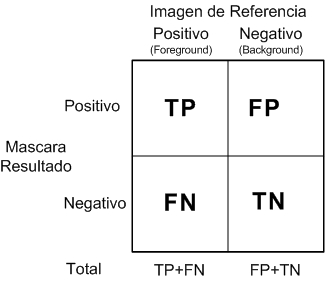
\includegraphics[scale=0.6]{img/Confusion_Matrix}
\caption{Matriz de Confusión}
\label{fig:confusion_matrix}
\end{figure}

Una condición positiva de la imagen de referencia en esta tabla, se refiere a todos los píxeles que circunscriben la silueta (\emph{foreground}) que un algoritmo debiera separar del fondo de imagen, y la condición negativa son todos los píxeles que están en el fondo de la imagen. En otro aspecto, la condición positiva en el resultado de la separación (mascara) son todos los píxeles que fueron clasificados pertenecientes a la silueta, y la condición negativa son todos los píxeles clasificados en la imagen de fondo. Los números localizados en la diagonal principal de esta matriz representan decisión correcta ($TP$ y $TN$) y los números de diagonal opuesta ($FN$ y $FP$) son los errores (``confusión'') realizados durante la clasificación, en este caso son los errores del algoritmo al equivocar píxeles de la imagen de fondo con píxeles de la silueta y píxeles de una silueta con los de la imagen de fondo.

\[
Precision=\frac{Total \: pixeles \, en \, foreground \, clasificados \, correctamente}{Total \, pixeles \, imagen \, resultante}
\]\\
\[
Recall=\frac{Total \: pixeles \: foreground \, clasificados \, correctamente}{Total \, foreground \, pixeles \, de \, imagen \, referencia}
\]\\
\[
True Positive Rate=\frac{Positivos  \: (silueta) \: clasificados \, correctamente}{Total \, positivos}
\]\\
\[
False Negative Rate=\frac{Negatives  \: (background) \: clasificados \, incorrectamente}{Total \, negativos}
\]

A partir de esta matriz de contingencia, se determinan una serie de métricas comunes de calidad, que se utilizan en los algoritmos de clasificación. La \textbf{tasa verdaderos positivos} (\textit{true positive rate}) es una medida de proporción de los positivos (píxeles de la silueta) seleccionados correctamente, está métrica también es conocida como \textit{recall} o \textit{sensitivity}. La \textbf{tasa falsos positivos} (\textit{false positive rate}) o tasa de falsas alarmas, corresponden a la proporción de negativos (píxeles \textit{background}) clasificados incorrectamente. Una medida complementaria a la tasa de falsos positivos es la métrica de \textit{specificity}, el cual es una proporción de negativos (\textit{background}) clasificados correctamente. En sistemas de recuperación de información (\emph{Information Retrieval}) las medidas de \emph{precision} (medida de proporción de la cantidad de píxeles seleccionados correctamente), \emph{recall} y media armónica \emph{F-Measure} \cite{brutzer_evaluation_2011} \cite{herrero_background_2009} \cite{park_benchmark_2013} (medida de desempeño total) son muy utilizadas como métricas de evaluación de rendimiento.



\begin{equation} \label{eq:precision}
Precision = \frac{TP}{TP + FP}
\end{equation}
\begin{equation} \label{eq:tpr}
True \: Positive \; Rate = \frac{TP}{TP+FN}
\end{equation}
\begin{equation} \label{eq:fpr}
False \; Positive \; Rate = \frac{FP}{FP + TN}
\end{equation}\\
\[
sensitivity = recall 
\]
\[
specificity = 1 - fpr
\]\\
\begin{equation} \label{eq:fmeasure}
F-Measure = \frac{1}{\frac{1}{precision} + \frac{1}{recall}}
\end{equation}

\begin{figure}
\centering     %%% not \center
\subfigure[Mascara estimada]{\label{fig:mask}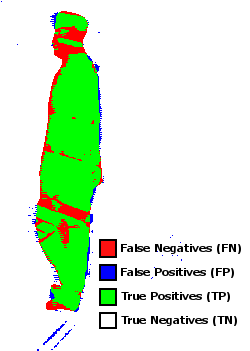
\includegraphics[width=50mm]{img/mask}}
\subfigure[Imagen de referencia]{\label{fig:gt}
\includegraphics[width=50mm]{img/gt}}
\label{fig:metricas_calidad_estatica}
\caption[Métricas de calidad estática]{Métricas de calidad estática, imagen de referencia y mascara estimada por algoritmo}
\end{figure}


\subsection{Curva de operaciones característica}
Los algoritmos de sustracción de imágenes de fondo o separación de \emph{foreground} y \emph{background}, son métodos que clasifican un píxel perteneciente a la imagen de fondo o a un objeto que está en movimiento, como una silueta del actor (\emph{foreground}). La curva de operaciones características (\textit{receiver operating characteristics - ROC}) es un gráfico que permite visualizar en forma global el desempeño de clasificación de un algoritmo. Un punto en esta curva relaciona la respuesta de clasificación, en este caso proporción de píxeles clasificados correctamente, con la proporción de píxeles negativos incorrectos. Describe un balance relativo entre beneficios (\emph{verdaderos positivos}) y costos (\emph{falsos positivos}). La curva se construye con el resultado de varias operaciones distintas, utilizando el mismo conjunto de datos, pero modificando algún parámetro característico de este algoritmo. Esto permitiría comparar el desempeño con diferentes configuraciones de un algoritmo.

La figura \ref{fig:tpr_fpr} es una curva ROC de ejemplo, que muestra el resultado de dos algoritmos distintos que están siendo comparados. El punto (0,0) de la esquina inferior izquierda representa una estrategia de nunca producir una clasificación positiva, un algoritmo localizado en este punto no genera errores de falso positivo, pero tampoco obtiene verdadero positivos. El punto (1,1) es opuesto al anterior, siempre tiene clasificaciones positivas. El punto (0,1) es el resultado de clasificación perfecta, los píxeles en foreground fueron detectados completamente, sin errores en los píxeles de la imagen de fondo. Un punto en el espacio ROC es mejor que otro, sí esta localizado más cerca de la esquina superior izquierda que el otro punto; el algoritmo presenta una tasa de verdaderos positivos alta y una tasa de falsos positivos baja. Algoritmos que se ubican en la parte izquierda del gráfico, cercano al eje X, se pueden considerar ``convervadores'', hacen una clasificación positiva teniendo buena evidencia, tienen muy poco errores de falso positivo, pero tienen también una baja tasa de verdaderos positivos. Al contrario, algoritmos que se ubican en la parte superior derecha de la gráfica, son algoritmos más libres, hacen clasificaciones positivas con poca evidencia, clasificando todos los positivos correctamente, pero con una alta tasa de falsos positivos. 




\begin{figure}[!ht]
\centering
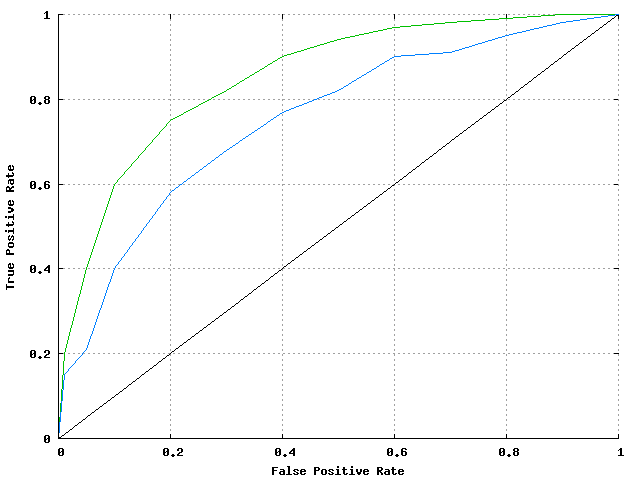
\includegraphics[scale=0.5]{img/curva_operaciones_caracteristicas}
\caption{Curva de operaciones características}
\label{fig:tpr_fpr}
\end{figure}




\subsection{Métricas de Percepción}

Estas métricas intentan ponderar el concepto de percepción de un observador, sobre el resultado final de segmentación. Se propone cuantificar los conceptos de \emph{exactitud espacial} (spatial accuracy) y \emph{estabilidad temporal} \cite{liu_metrics_2011} \cite{cavallaro_objective_2002} o \emph{coherencia temporal} \cite{villegas_perceptually-weighted_2004}. Ponderan, mediante algún tipo de función definida, la discrepancia entre una mascara estimada y la de su referencia (ground-truth), tomando en cuenta la inexactitud potencial que puede contener la mascara de referencia, la localización de los pixeles con errores relativo al borde de la mascara de referencia, y el tipo de errores (FP, FN). 

\subsubsection{Contexto espacial y temporal}
El contexto espacial \cite{cavallaro_objective_2002} de un pixel errado, es caracterizado por la distancia más cercana de un objeto detectado. Esta propiedad relaciona el foco de atención de un observador hacia a un objeto que le llama la atención, errores del tipo falso negativo (pixel clasificado erróneamente como foreground) son más importantes en la medida que la distancia es mayor. El contexto temporal considera las diferencias de calidad en el tiempo, para esto identifican dos tipos de fenómenos; un efecto sorpresa y un efecto fatiga. El efecto sorpresa se relaciona con los cambios en la exactitud espacial y el efecto fatiga se relaciona con el hecho de un observador se acostumbra a cierto tipo de calidad en el tiempo. Estos dos contextos son relacionados en las siguientes expresiones.

\begin{equation}
\nu_w(n) = 1 - \epsilon_w(n)
\end{equation}

\begin{equation}
\zeta_w(n) = \frac{\nu_w(n)}{2} \lbrack 1 + \alpha_t \frac{d}{dn}\nu(n) \rbrack
\end{equation}

Siendo $\nu_w(n)$ un valor de ponderación de la exactitud espacial, $\frac{d}{dn}\nu(n)$ variación espacial en el tiempo (mientras mayor esta variación más pequeño su coherencia temporal) y $\zeta_w(n)$ una medida de calidad de percepción espacial-temporal. Se define una \emph{exactitud espacial absoluta} y \emph{relativa} (normalización por el total de pixeles) como la contribución de las ponderaciones de $w^i_p$ (falso positivo), y $w^j_n$ (falso negativo) . 

\begin{equation}
w^i_p = \frac{\alpha_p \log(d^i_p + 1)}{D}
\end{equation}

\begin{equation}
w^i_j = \frac{\alpha_nd^j_n}{D}
\end{equation}

\begin{equation}
\epsilon_w() = \sum_{i=1}^{\epsilon_p(n)}w^i_p +	 \sum_{j=1}^{\epsilon_n(n)} w^j_n
\end{equation}


\begin{figure}[!ht]
\centering
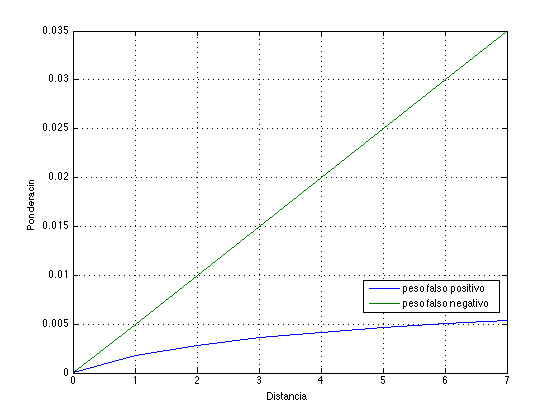
\includegraphics[scale=0.4]{img/PesosFalsoPositivoNegativo}
\caption{Pesos pixeles falso positivo y negativo}
\label{fig:Contexto espacial pesos para pixeles falso positivo y negativo}
\end{figure}

Como se indica en la figura 2, ambas ponderaciones o pesos $w^i_p$ y $w^j_n$ aumentan con la distancia, pero influyen en forma diferenciada en la ponderación final de exactitud espacial. Los pesos para falsos positivos se incrementan en forma lineal, y estos valores son mayores con los pesos de los falsos negativos a la misma distancia.

\subsubsection{Observaciones para cuantificación espacial}

Las mediciones de exactitud espacial del trabajo propuesto en \cite{liu_metrics_2011}, se basan en observaciones que toman en consideración, el error producido al generar las mascaras de referencia en forma manual. Se menciona que los pixeles errados, muy cerca de los bordes de las mascaras de referencia, se presumen causados por la inexactitud durante la creación de estas mascaras. A su vez, una segunda observación indica que estos mismos errores muy cercanos al borde, tienen poco efecto comparado con otro que se encuentra muy lejano del borde. Pese a que estos pixeles en el borde hacen que un objeto parezca más grueso o delgado, estos no cambian la forma del objeto. Una tercera observación, señala que el impacto de los diferentes tipos de errores durante el procesamiento no son similares, por lo que hacen las distinción de medir en forma independiente falsos negativos y falsos positivos. 

Se propone una función ponderación del tipo sigmoidal, de esta forma errores muy cercanos al borde de la mascara tienen un valor (peso) menor a uno y otros errores lejanos al borde se aproximan a uno. 

\begin{equation}
S(d;\alpha) = \frac{1 - e^{-\alpha \cdot d}}{1 + e^{-\alpha \cdot d}}
\end{equation}

Esta función $S$, tiene como variable $d$ distancia de un pixel en error al borde de la mascara, y $\alpha$ es parámetro que modela la tolerancia de la inexactitud de las mascaras de referencia en sus bordes. Un parámetro $\alpha$ pequeño conlleva una capacidad de tolerancia mayor. 

\begin{figure}[!ht]
\centering
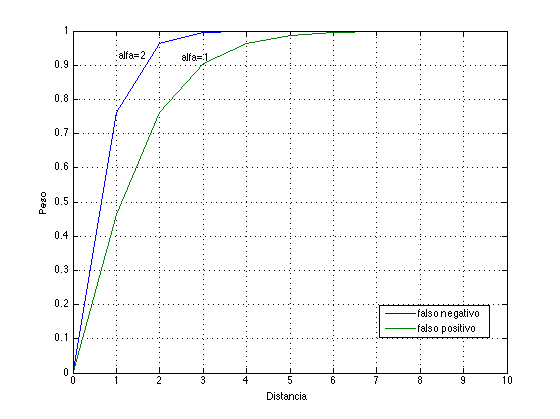
\includegraphics[scale=0.4]{img/sigmoid_function}
\caption{Pesos usando función tipo sigmoidal}
\label{fig:Pesos tipo sigmoidal}
\end{figure}


\subsection{Similaridad Estructural}
El índice de \emph{similaridad estructural} - \emph{SSIM} (\emph{Structural SIMilarity}) \cite{park_benchmark_2013} \cite{wang_image_2004} es un método de medición de similaridad entre dos imágenes. Es una medida de calidad de una imagen de entrada contrastada con otra de buena calidad. Este índice usa un nuevo enfoque para medir calidad, se basa en la hipótesis que la principal función del ojo humano  es extraer información estructural de su campo visual, y además el Sistema Visual Humano (\emph{Human Visual System - HVS}) está muy adaptado para realizar esta operación. Por lo tanto una medición de distorsión estructural podría ser una buena aproximación. Se platean entonces, en este nuevo enfoque, moverse desde mediciones de errores (métodos vistos anteriormente) a realizar mediciones de distorsión estructural. Sin embargo, el nuevo problema que se debe enfrentar es cómo definir y cuantificar distorsiones estructurales.

El modo de medir y obtener el índice \emph{SSIM} supone una secuencia de imágenes de entrada en escala de grises además de la secuencia de imágenes de referencia, ground-truth. Se considera la secuencia de referencia como la secuencia con las imágenes de buena calidad, de esta forma la medida de similaridad sirve como una medición de la calidad de la otra secuencia de entrada. La manera de medir similaridad es separar la tarea en tres componentes; \emph{luminancia}, \emph{contraste}, y \emph{estructura}.

\begin{equation}
SSIM(x,y) = f(l(x,y), c(x,y),s(x,y)) 
\end{equation}

\begin{equation}
SSIM(S,G) = (\frac{2\mu_S\mu_G + c_1}{\mu_S^2 + \mu_G^2 + c_1}) \cdot (\frac{2\sigma_S\sigma_G + c_2}{\sigma_S^2\sigma_G^2 + c_2}) \cdot (\frac{\mu_{SG} + c_3}{\mu_S\mu_G + c_3})
\end{equation}

Este índice de calidad es una combinación de tres factores, pérdida de correlación, distorsión media, y varianza de la distorsión. El primer componente es el coeficiente de correlación lineal entre $S$ y $G$ y su rango dinámico varia en $[-1,1]$. El segundo componente mide similaridad entre valores medios, y su rango de valores está entre $[0,1]$. El tercer componente mide similaridad entre las varianzas de ambas imágenes de una secuencia, y su rango dinámico está entre $[0,1]$. La relación final aplicada sobre secuencia de vídeo viene dada por la siguiente formula. 


\begin{equation}
SSIM(S,G) = \frac{1}{n} \sum_{i=1}^{n} \frac{(2\mu_{S_{i}} \mu_{G_{i}} + c_1) \cdot (2 cov_{S_iG_i} + c_2)}  {(\mu^2_{S_i} + \mu^2_{G_i} + c_1) \cdot (\sigma^2_{S_i} + \sigma^2_{G_i} + c_2)}
\end{equation}

Donde, $S$ es un conjunto de $n$ imágenes resultantes, $G$ conjunto de las imágenes de referencia (ground-truth), $\mu_{S_i}$ $\mu_{G_i}$ media de ambas secuencias, $\sigma_{S_i}$ y $\sigma_{G_i}$ desviaciones estándar, y $cov_{S_iG_i}$ covarianza de $S_i$ y $G_i$. Las constantes $c_1 = (k_1 + L)^2$ $c_2=(k_2 + L)^2$ con valores $k_1=0.01$ $k_2=0.03$ y $L=255$.


\subsection{D-Score}
D-Score brinda un criterio de \emph{disimilitud} entre una imagen de referencia y la imagen de entrada, esta métrica sólo considera fallas en la medición de los resultados. El costo de un error depende de la distancia con el objeto más cercano de la referencia, teniendo una ponderación mayor los errores en el rango intermedio. Esto debido que este tipo de errores impactan de mayor manera el reconocimiento de formas. Por ende, errores en zonas lejanas/cercanas tendran un D-score cercano a cero. 

\begin{equation}
DT(x) = min( d(p,x), \forall x \in X)
\end{equation}

El costo de error se basa en una \emph{Tranformada de Distancia} (Distant Transform - DT) de la referencia ground-truth, con $X$ un conjunto de pixeles de referencia, $d(p,x)$ es la distancia del pixel $p$ al pixel $x$, entonces $DT(x)$ es la distancia mínima entre un pixel $x$ y el punto de referencia más cercano. Para calcular $DT(x)$ se usa la siguiente relación

\begin{equation}
D-score(x) = exp( - (\log_2(2.DT(x)) - \alpha )^2)
\end{equation}


\begin{figure}[!ht]
\centering
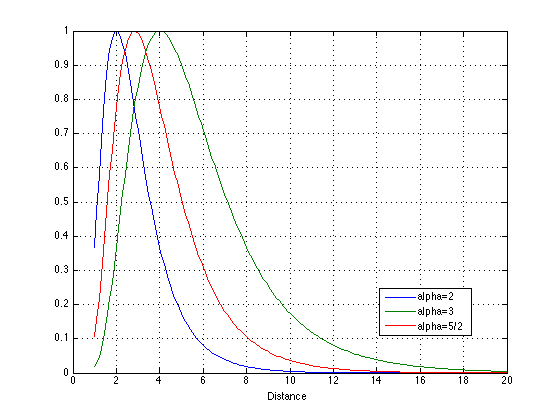
\includegraphics[scale=0.4]{img/dscore}
\caption{Valores D-Score basados en la distancia desde la referencia ground-truth}
\label{fig:Valores D-Score}
\end{figure}

De acuerdo con la figura 4, se tiene una tolerancia de 3 pixeles desde la referencia, esto debido que ese tipo de errores locales no afecta realmente el proceso de reconocimiento. De esta misma forma tomando un valor de $\alpha=5/2$, \cite{park_benchmark_2013}, se permiten que ocurran errores a más de 10 pixeles de distancia. D-score entrega un índice que señala el nivel de reconocimiento de objetos, en la medida que este valor es menor, mejor es el reconomiciento, independiente del valor de errores que entreguen otros índices, como el \emph{F-Measure}.

\section{Resumen de métodos de evaluación}
Se ha hecho una descripción de la mayoría de los métodos de medición utilizados actualmente, basados principalmente en el paradigma de evaluación por discrepancia  o error. Una menor discrepancia con una referencia, brindan un ranking de mayor calidad de clasificación o comparación de algoritmos. En general, no existe una métrica ideal, que pueda ser utilizada como herramienta de comparación universal, entre los diferentes algoritmos existentes. De igual modo, estas métricas pueden ser empleadas en conjunto, de manera complementaría, aprovechando las diferentes características de ellas. Un caso concreto es el trabajo desarrollado para el desafío BMC \cite{park_benchmark_2013}.

Las métricas más empleadas sin duda son ``specificity'' ($1-fp\; rate$), ``sensitivity'' (recall) y todas sus demás variantes, estas métricas proporcionan una medida general del resultado de clasificación. Presentan el compromiso entre la habilidad del algoritmo para identificar los píxeles correspondientes a una silueta (\emph{sensitivity}), y la habilidad del mismo algoritmo para identificar los píxeles pertenecientes a la imagen de fondo (\emph{specificity}). Estas dos métricas se colocan en una curva de ROC que permite comparar desempeño con otro algoritmo bajo las mismas condiciones. 

Las diferentes métodos basadas en el concepto de percepción se aproximan a una forma de evaluación que podría hacer un observador humano, para esto, hacen una combinación de un contexto espacial con un contexto temporal. Los errores se ponderan de acuerdo con distancia al borde de la mascara de referencia, la estabilidad de esta percepción espacial es además considerada en la evaluación de calidad. Los distintos enfoques encontrados de esta metodología se diferencian en el tipo de función empleada para hacer la ponderación espacial de los errores con respecto a la distancia del borde de su mascara. Evalúan con mayor ponderación el error falso negativo y localizado lejano al borde de la mascara. La métrica de ``D-Scorre'', a diferencia de la descripción previa castiga fuertemente los pixeles errados en el borde de la mascara, porque este tipo de errores no permiten realizar una buena clasificación.

Un diferente enfoque presenta el índice de similaridad, este ya no utiliza las mediciones de percepción para evaluar calidad. Postula medición de distorsión estructural, para esto se propone una combinación de mediciones de luminancia, contraste y estructura. Que vienen siendo análisis de correlación entre dos imágenes, cuantificación de sus varianzas y sus medias. 

Finalmente, estas distintas métricas pueden ser empleadas en conjunto o en forma individual. Pero una combinación de ellas podría brindar una mejor claridad desde el punto de vista de la calidad de los diferentes algoritmos. Pueden entregar una mejor discriminación de las ventajas y falencias en diversas condiciones ambientales. Se podría determinar un buen algoritmo para ciertas condiciones, pero también determinar sus desventajas en otras situaciones. 





